\chapter{Spiking Neural Networks~(SNNs)}
\label{cha:bkg}
This chapter aims to introduce fundamental concepts of spiking neurons, which are basic processing units of SNNs, and all the proposed work in the thesis will be built on such units.
Hence, we will start from the elementary neuroscience notions in Section~\ref{sec:neuron_basic} to give a general impression of a spiking neuron and neural signals propagated among network of neurons.
These neural signalling dynamics can be abstracted and simplified by mathematical models, for example leaky integrate-and-fire~(LIF) model, which will be a popular neural model used in our research.
Thus, Section~\ref{sec:spike} will present neural dynamic modelling by taking the example of LIF neurons, and a modelled biological-plausible learning rule.
To operate networks of spiking neurons, in Section~\ref{sec:snn_sim} we will introduce the simulators both in software and hardware, including neuromrophic systems.


%The so-called third generation of neural networks~\cite{maass1997networks} introduces a different set of functions and parameters to model neurons;
%%these both model biological neurons more precisely~\cite{hodgkin1952quantitative} and increase the computational power of networks of neurons if compared to classical sigmoidal units.
%it models the biological neurons more precisely and increases the computational power of neural networks when compared to the classical sigmoid functions.
%Such networks rely on the propagation of an all-or-none signal, the action potential, which asynchronously carries information to its connected units by means of its timing.
\section{Neural System Basics}
\label{sec:neuron_basic}

	\begin{figure}[bt]
		\centering
		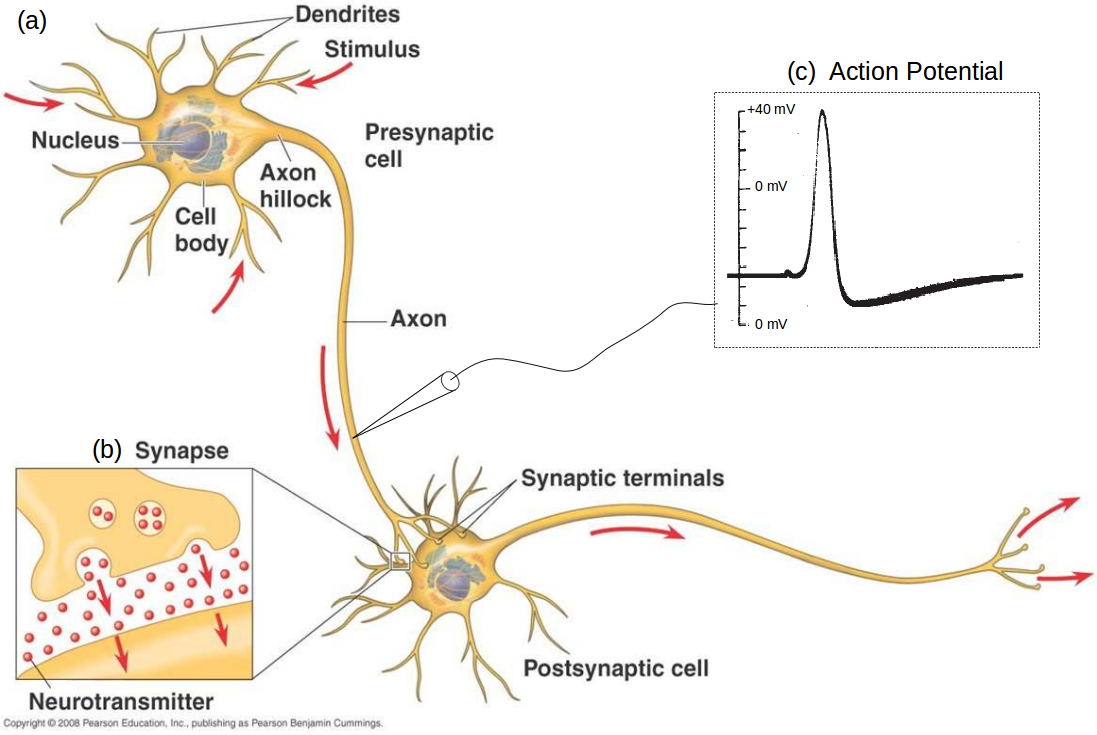
\includegraphics[width=0.98\textwidth]{pics_snn/neuron2.png}
		\caption{Two neurons connected by synapses. 
			A neuron mainly is composed of three functional parts: dendrites, the soma, and the axon. (a) A Presynaptic cell connects to its postsynaptic cell through synapses~\cite{reece2011campbell}, see (b)~\cite{reece2011campbell}, and the neural signal, action potential see (c)~\cite{hodgkin1939action}, propagates along the red arrows. }
		\label{Fig:neuron_basic}
	\end{figure}

\subsection{Biological Neural Components}
%\subsubsection{Neurons}
What composes a spiking neuron?
%Spiking neuron models can be divided into two major categories \cite{gernstbook} based on their level of abstraction: The conductance models and the threshold models.
%The conductance models simulate a lower level on the ion channels, while the threshold models represent a higher level of neuron abstraction where the threshold voltage is fixed and the neuron fires once the membrane potential reaches it.
%
%In general, Conductance-Based models have been derived from the Nobel prize winners (1963) Hodgkin and Huxley, based on the experiments that they performed on the giant axon squid \cite{hhmodel}.
%Spikes arriving at a LIF neuron cause a temporary flow of current into (excitatory synapse) or out of (inhibitory synapse) the neuron, modelling the behaviour of synapses in biological neurons.
%The LIF neuron sums up this current over time, accumulating charge which gradually leaks away.
%If the membrane potential in the neuron reaches a certain threshold, it produces a spike and its charge is reset.
%LIF neurons have been extensively used in large spiking neural networks \cite{Delorme1999989} because of their ease of implementation and the low computational cost.

%\subsubsection{Spikes}

%\subsubsection{Synapses}

\subsection{Neuronal Signals}

What is the signal transited among neurons?
and what are the codes.

%Code:https://www.slideshare.net/ieee_cis_cyprus/jennie-si
\subsubsection{Action Potential}
\begin{figure}[bt]
	\centering
	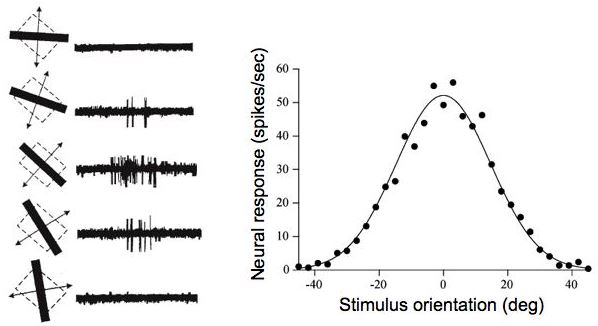
\includegraphics[width=0.8\textwidth]{pics_snn/v1.jpg}
	\caption{Example of rate coding: cat V1~\cite{hubel1962receptive}.}
	\label{Fig:v1}
\end{figure}

\begin{figure}[bt]
	\centering
	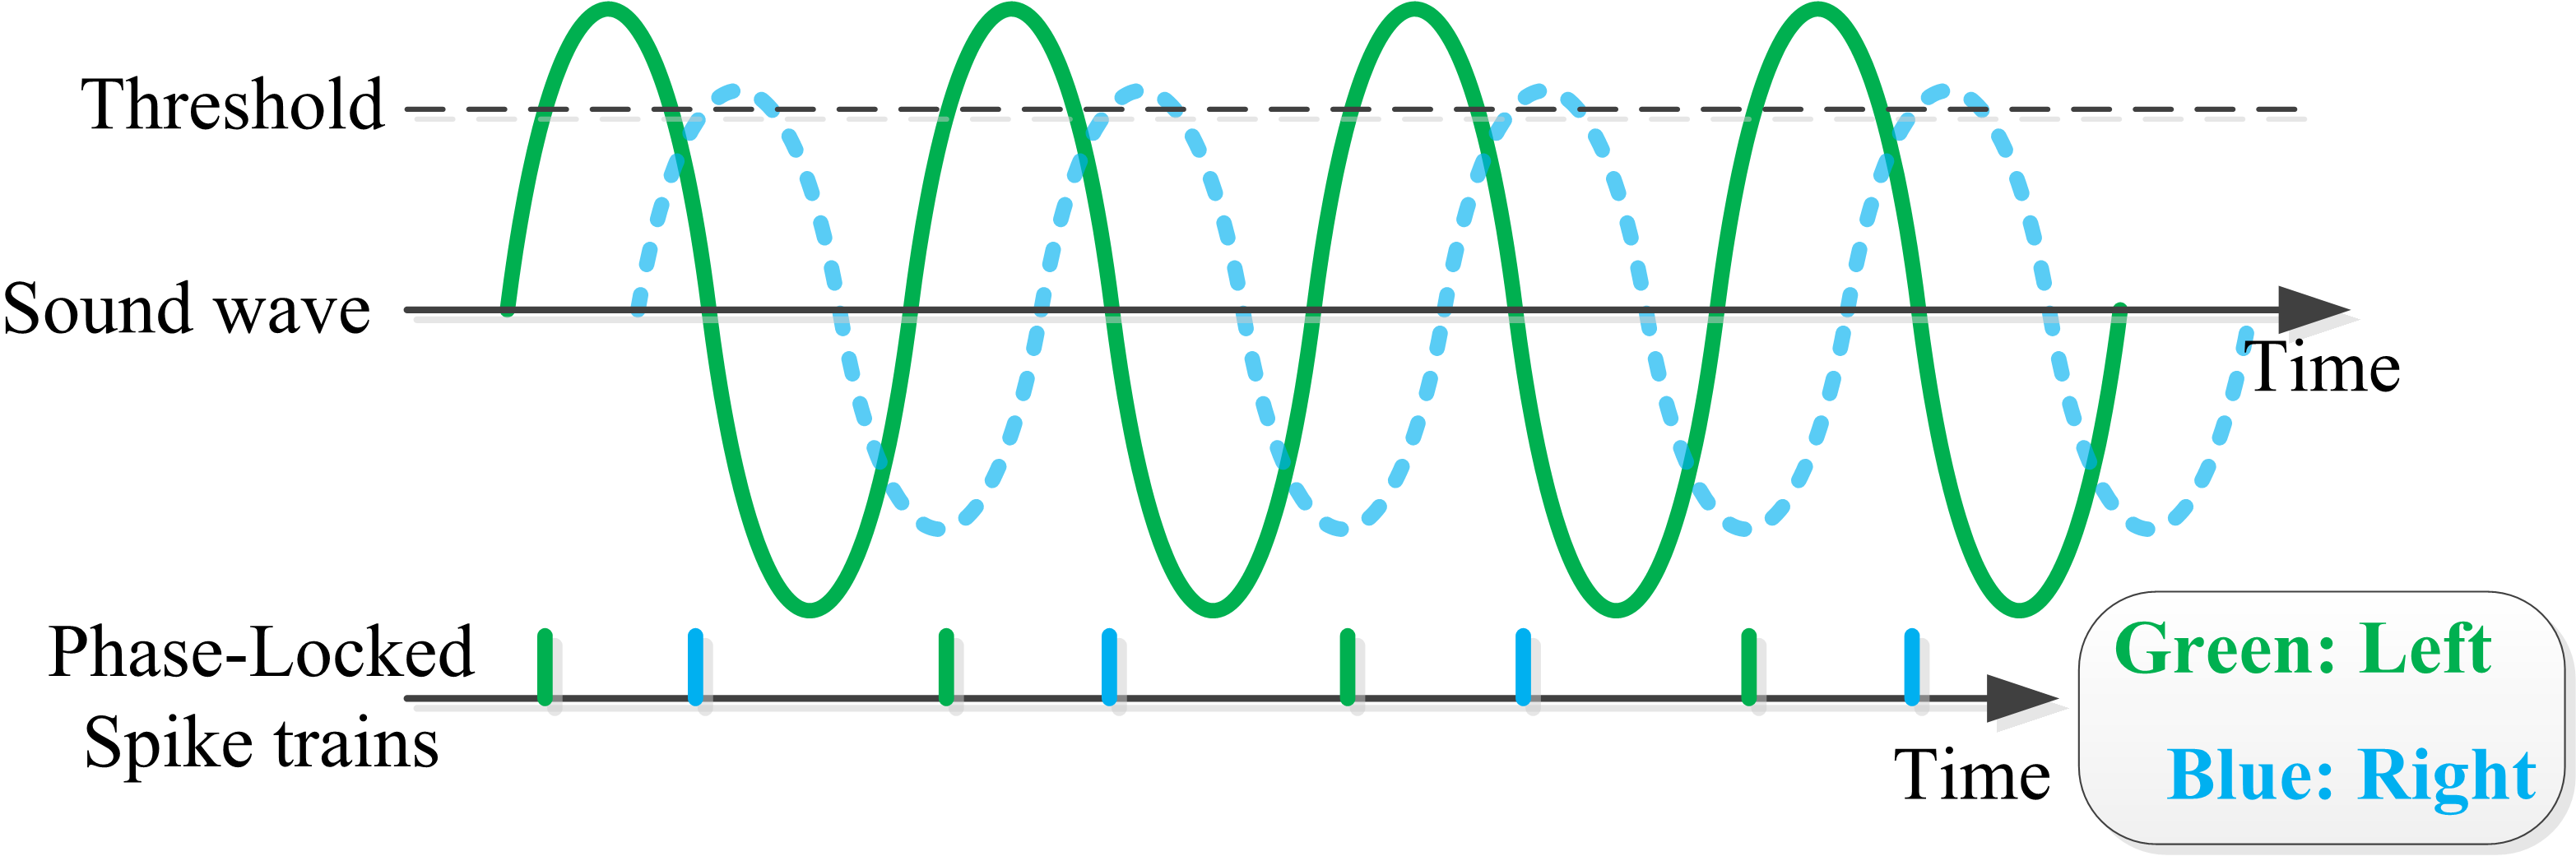
\includegraphics[width=0.8\textwidth]{pics_snn/phaselocking.png}
	\caption{Example of temporal coding: auditory fibre~\cite{liu2013modeling}.}
	\label{Fig:audio_fibre}
\end{figure}

\subsection{Signal Transmission}
How these signals are propagated? 
\subsubsection{Synapse}




\section{Modelling Spiking Neurons}
\label{sec:spike}
\subsection{Neural Models}
\subsubsection{Membrane Potential}
\begin{figure}[bt]
	\centering
	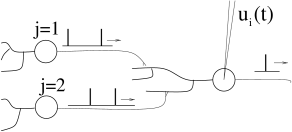
\includegraphics[width=0.6\textwidth]{pics_snn/x10.png}
	\caption{An electrode measures the membrane potential of a postsynpatic neuron~\cite{gerstner2014neuronal}.}
	\label{Fig:mem_potential}
\end{figure}

\subsubsection{Postsynaptic Potential}
PSP
\begin{figure}[bt]
	\centering
	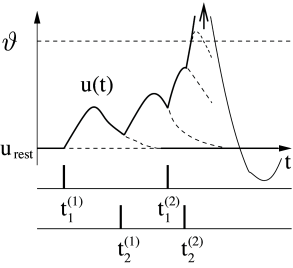
\includegraphics[width=0.6\textwidth]{pics_snn/x11.png}
	\caption{A postsynpatic neuron receives input from two neurons which fires at time $t$~\cite{gerstner2014neuronal}.}
	\label{Fig:psp}
\end{figure}

\subsection{Synaptic Models}
\subsection{Synaptic Plasticity}


\begin{figure}[bt]
	\centering
	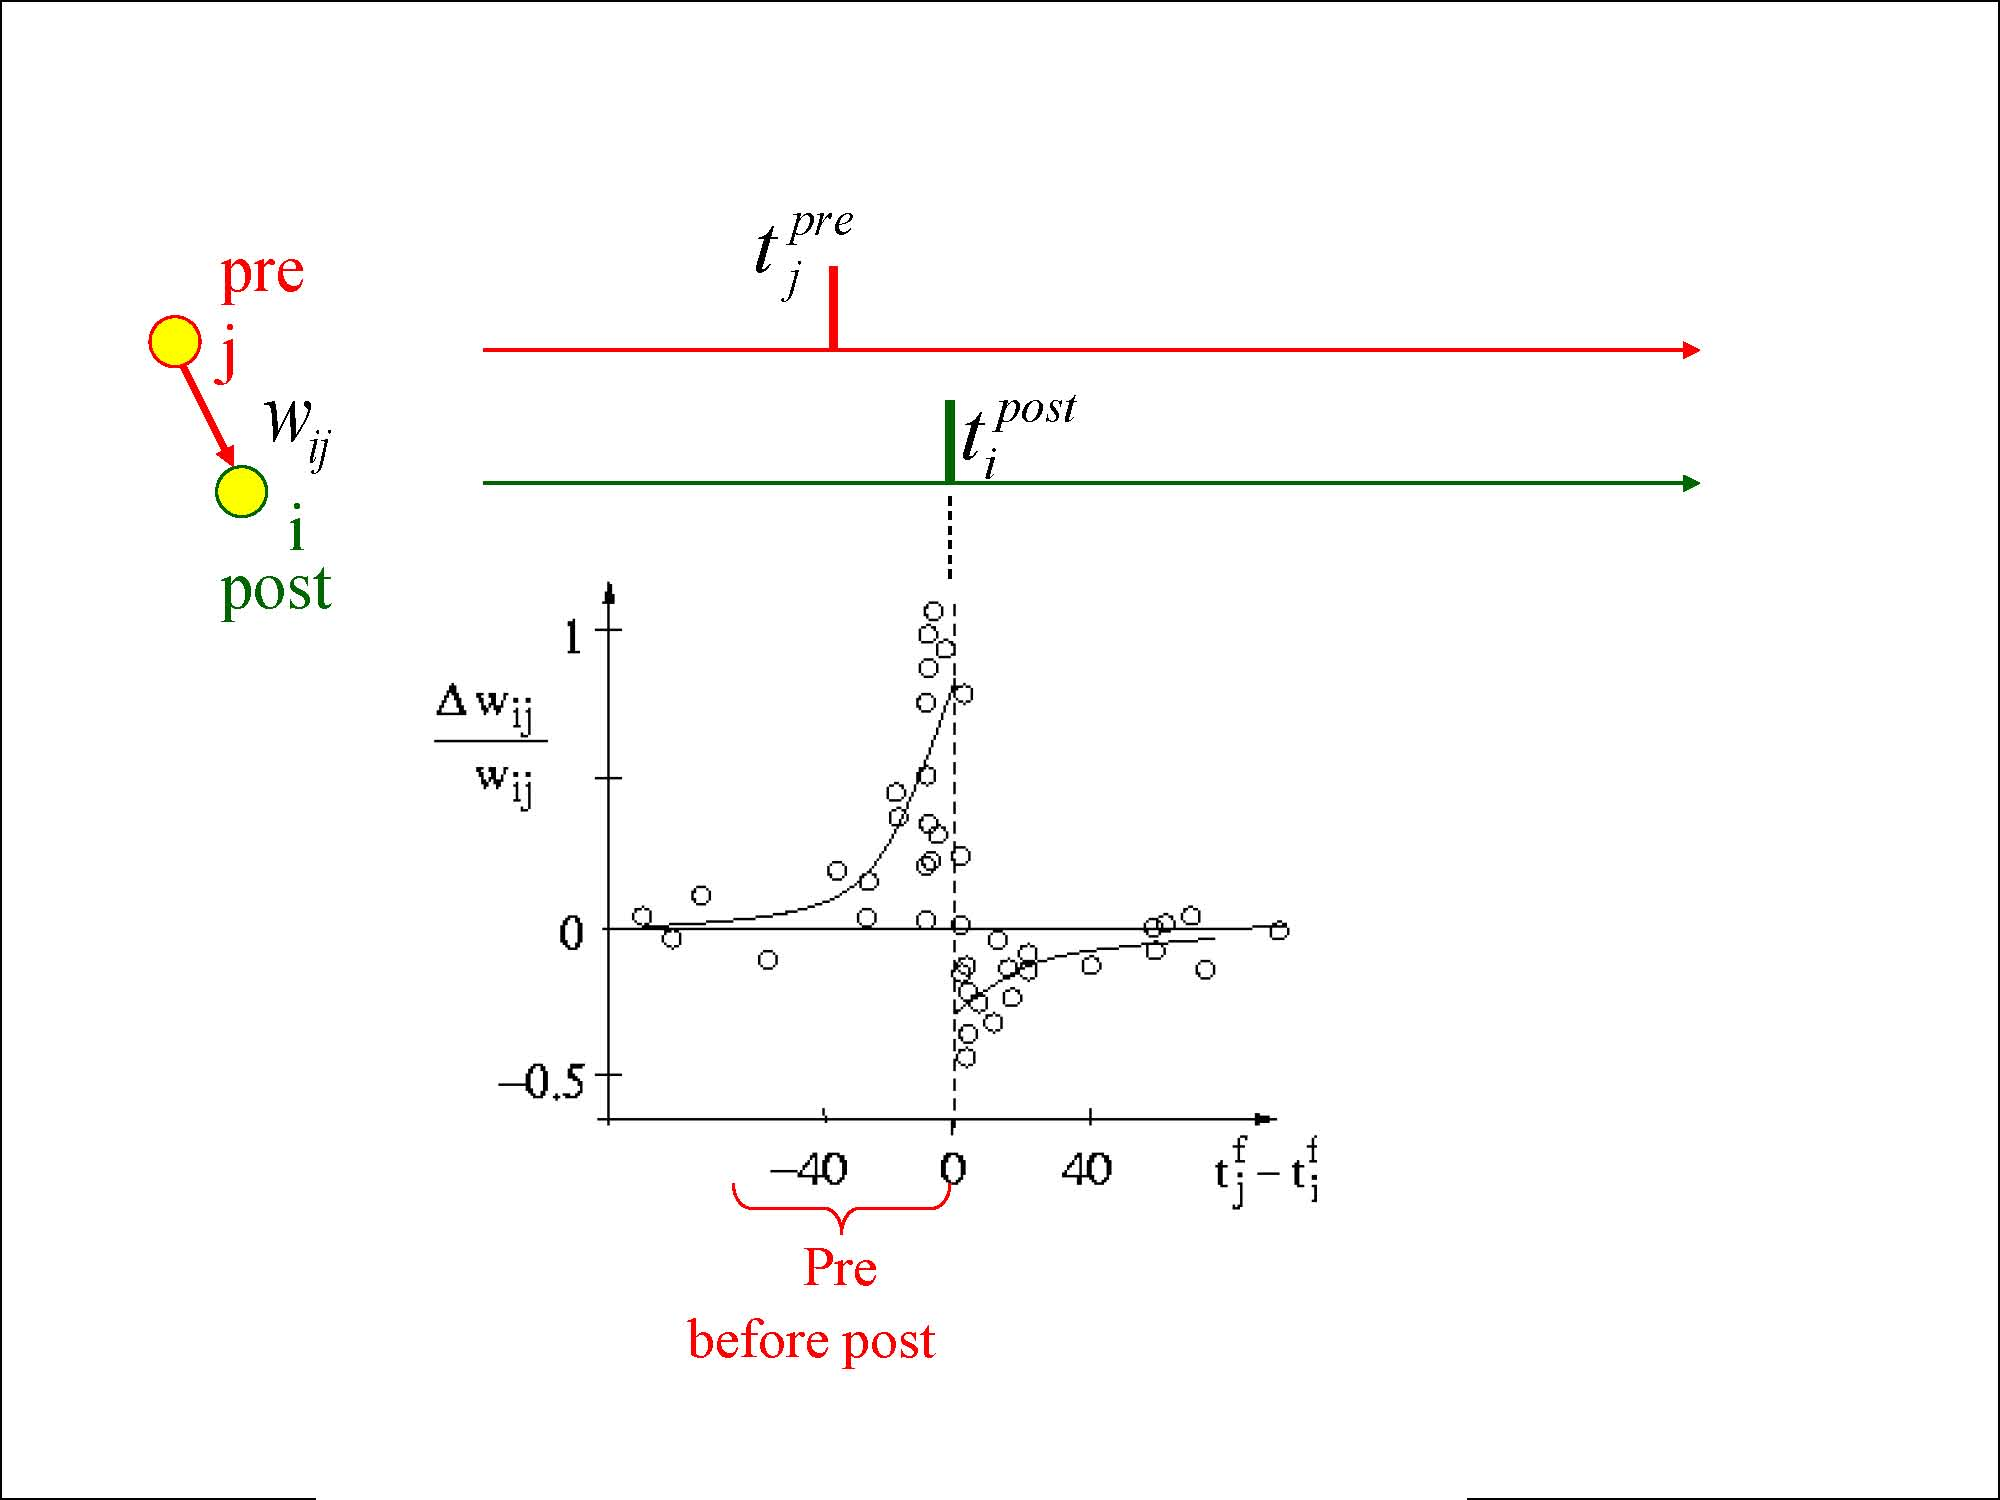
\includegraphics[width=0.8\textwidth]{pics_snn/fig_stdp_orig.jpg}
	\caption{Synaptic Time Dependant Plasticity~\cite{gerstner2014neuronal}.}
	\label{Fig:STDP}
\end{figure}
%One of the key parameters of a neural network is the amount of influence each incoming spike has on a neuron.
The influence each incoming spike has on a post-synaptic neuron is modelled by assigning a `weight' to each synapse;
tuning on the weight scales the impact of a spike
arriving via that synapse.
Many learning models simulate the changes in weights over long periods of time observed within the brain.
The exact rules by which these weights are adjusted is the subject of much active research though most promising approaches attempt to learn from the relative timing \cite{pfister2006triplets} or rate \cite{bienenstock1982theory} of spikes arriving at a neuron.
As well as adjusting weights, some learning rules can also form entirely new connections between previously unconnected
neurons \cite{bamford2010synaptic}.

\section{Simulating Networks of Spiking Neurons}
\label{sec:snn_sim}
\subsection{Software Simulators}
\subsection{Hardware Simulators}
\subsection{Neuromorphic Systems}
\label{sec:morph}

